\section{高次不等式的解法}

不等式$(x-x_1)(x-x_2)\cdots(x-x_n)>0$
(其中$x_1,x_2,\ldots,x_n$是互不相等的实常数)是一元$n$次不等式($n\in\N$). 

若$n=1$,容易写出它的解集为$(x_1,+\infty)$;

若$n=2$,它是一元二次不等式。只要能正确地作出相应的二次函数的图象的草图(关键是开口方向和函数的零点不能弄错),再根据图象写出不等式的解集就没有什么困难了。现在的问题是,能否把这种解法——图象法,推广到$n\ge 3$的情况。

很明显,这时关键在于怎样作出相应函数的图象的草图,让我们先剖析一个实例——作出下列函数图象的草图:
\[y=f(x)=(x+1)(x-1)(x+5)\]

第一步,曲线$y=f(x)$与$x$轴的交点的横坐标(称为\textbf{函数$y=f(x)$的零点})由小到大依次是$-5$,$-1$,1,此时$x$轴被这三个交点分成四段,它们分别对应四个开区间:
\[(-\infty,-5),\quad (-5,-1),\quad (-1,1), \quad (1,+\infty)\]

第二步,研究曲线$y=f(x)$在这四个开区间上分布在横轴的上方还是下方:

在$(1,+\infty)$上,由于$x>1$,所以$x+1>0$, $x-1>0$, $x+5>0\Longrightarrow y>0 \Longrightarrow $曲线$y=f(x)$在$x$轴上方;

在$(-1,1)$上,由于$-1<x<1$,所以$x+1>0$, 
$x-1<0$, $x+5>0\Longrightarrow y<0\Longrightarrow $ 曲线$y=f(x)$在$x$轴下方;

在$(-5,-1)$上,由于$-5<x<-1$,所以$x+1<0$, 
$x-1<0$, $x+5>0\Longrightarrow y>0\Longrightarrow$ 曲线$y=f(x)$在$x$轴上方;

在$(-\infty,-5)$上,由于$x<-5$,所以$x+1<0$, $x-1<0$, $x+5<0\Longrightarrow y<0\Longrightarrow$曲线$y=f(x)$在$x$轴下方;

规律性很明显:曲线$y=f(x)$在上述四个彼此相邻的开区间内,从右到左依次位于$x$轴的上方、下方、上方、下方,而在$x=-5,-1,1$三处曲线与$x$轴相交。

第三步,根据上述分析,作出函数图像的草图(图4.5)。

\begin{figure}[htp]
    \centering
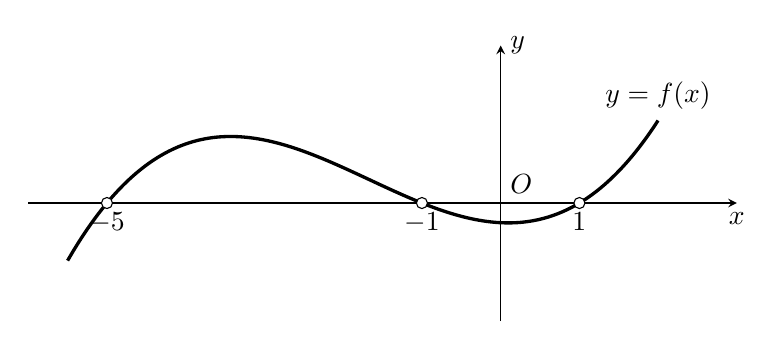
\begin{tikzpicture}[>=stealth]
\draw[->](-6,0)--(3,0)node[below]{$x$};    
\draw[->](0,-1.5)--(0,2)node[right]{$y$};

\draw[domain=-5.5:2, smooth, samples=100, very thick]plot(\x, {0.05*(\x-1)*(\x+1)*(\x+5)})node[above]{$y=f(x)$};

\foreach \x in {1,-1,-5}
{
    \draw[fill=white](\x,0)node[below]{$\x$}circle(2pt);
}
\node [above right]{$O$};
\end{tikzpicture}
    \caption{}
\end{figure}


这种草图上要明确地表示出:
\begin{enumerate}[(a)]
    \item 曲线与$x$轴的交点;
    \item 在某个开区间上函数的那段曲线是在$x$轴的上方还是下方。
\end{enumerate}
除此以外,对草图不必做更细致的要求,例如在某个开区间上函数的最大值(最小值)画得是否确切等都无关紧要。因为在此处我们只关心不等式的解。

通过剖析实例,我们获得了作形如函数
$f(x)=(x-x_1)(x-x_2)\cdots (x-x_n)$
(其中$x_1,x_2,\ldots,x_n$是互不相等的实常数)
图像的草图的一般方法:

第一步,求出曲线$f(x)$与$x$轴交点的横坐标$x_1,x_2,\ldots,x_n$,并把它们由小到大依次标在$x$轴上。标出的$n$个点把$x$轴分成$n+1$个开区间。

第二步,因为曲线$y=f(x)$在这$n+1$个开区间上总是依次上下相间地分布在$x$轴两侧,而且在函数的零点处彼此相连。所以,我们只要确定曲线在最右边的开区间上分布在$x$轴的上侧还是下侧就行了。这是容易办到的,实际上我们总能使$x$的最高次幂的系数为正,曲线总是在$x$轴的上方。

第三步,根据上述分析,作出图象的草图。

\begin{example}
    解不等式:
    \begin{multicols}{2}
\begin{enumerate}[(1)]
    \item $(x-2)(x+1)(x+3)(x+5)>0$
    \item $(x+2)(x-3)(5-x)>0$
\end{enumerate}        
    \end{multicols}
\end{example}

\begin{solution}
\begin{enumerate}[(1)]
    \item 作出函数$y=(x-2)(x+1)(x+3)(x+5)$图象的草图(图4.6)

$\therefore\quad $不等式(1)的解集为$(-\infty,-5)\cup(-3,-1)\cup (2,+\infty)$

\begin{figure}[htp]
    \centering
\begin{minipage}{0.45\textwidth}
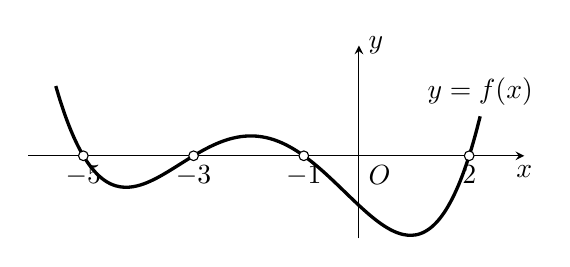
\begin{tikzpicture}[scale=.7, >=stealth]
\draw[->](-6,0)--(3,0)node[below]{$x$};    
\draw[->](0,-1.5)--(0,2)node[right]{$y$};

\draw[domain=-5.5:2.2, smooth, samples=100, very thick]plot(\x, {0.03*(\x-2)*(\x+1)*(\x+5)*(\x+3)})node[above]{$y=f(x)$};

\foreach \x in {-1,-3,-5,2}
{
    \draw[fill=white](\x,0)node[below]{$\x$}circle(2.5pt);
}
\node [below right]{$O$};


 \end{tikzpicture}
    \caption{}   
\end{minipage}\hfill 
\begin{minipage}{0.45\textwidth}
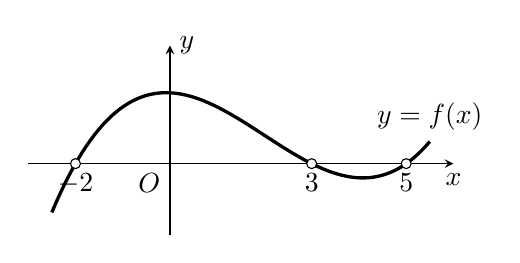
\begin{tikzpicture}[scale=.6, >=stealth]
    \draw[->](-3,0)--(6,0)node[below]{$x$};    
\draw[->](0,-1.5)--(0,2.5)node[right]{$y$};

\draw[domain=-2.5:5.5, smooth, samples=100, very thick]plot(\x, {0.05*(\x-3)*(\x+2)*(\x-5)})node[above]{$y=f(x)$};

\foreach \x in {-2,3,5}
{
    \draw[fill=white](\x,0)node[below]{$\x$}circle(3pt);
}
\node [below left]{$O$};


 \end{tikzpicture}
    \caption{}   
\end{minipage}
\end{figure}


\item 先把原不等式变成与它等价的$(x+2)(x-3)(x-5)<0$,作出函数$y=(x+2)(x-3)(x-5)$图象的草图(图4.7)

$\therefore\quad $解集为$(-\infty,-2)\cup(3,5)$.

\end{enumerate}

注意:在解题中,我们先以$(-1)$乘原不等式,为的是使因式$(5-x)$变成$(x-5)$。这样做可以避免出错。
\end{solution}

\begin{note}
这类不等式的解法可以概括成:找零点,分区间,画草图,写解集。
\end{note}

\begin{example}
解下列不等式:
\begin{enumerate}[(1)]
    \item $(x-4)(x-1)^2(x+2)<0$
    \item $(x+2)(x+1)^2(x-1)^3(x-3)>0$
\end{enumerate}
\end{example}

\begin{analyze}
    此例中函数的解析式$y=(x-4)(x-1)^2(x+2)$出现了重因式,当$x$值由大于1变到小于1的时候(不含$x=1$),$y$的取值符号没有发生变化,如图4.8所示.

\begin{figure}[htp]
    \centering
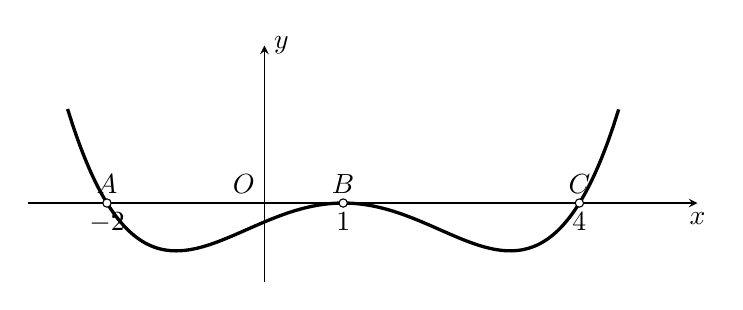
\begin{tikzpicture}[>=stealth]
    \draw[->](-3,0)--(5.5,0)node[below]{$x$};    
\draw[->](0,-1)--(0,2)node[right]{$y$};

\draw[domain=-2.5:4.5, smooth, samples=100, very thick]plot(\x, {0.03*(\x-4)*(\x+2)*(\x-1)*(\x-1)});

\foreach \x/\y in {-2/A,1/B,4/C}
{
    \draw[fill=white](\x,0)node[below]{$\x$}circle(1.5pt)node[above]{$\y$};
}
\node [above left]{$O$};
\end{tikzpicture}
    \caption{}
\end{figure}

    由此,不等式(1)的解集为$(-2,1)\cup (1,4)$.

    基于这个想法,不难得到:若$(x-x_1)$是曲线$y=f(x)$的二重因式,则曲线在点$B(x_1)$处不穿过横轴,若$(x-x_1)$是三重因式,则曲线在点$B(x_1)$处穿过横轴,依次类推。

    对于第(2)题,依上述办法作出函数$y=(x+2)(x+1)(x-1)^3(x-3)$的草图(图4.9).由此可得(2)的解集是$(2-1)\cup (-1,1)\cup (3,+\infty)$.

\begin{figure}[htp]
    \centering
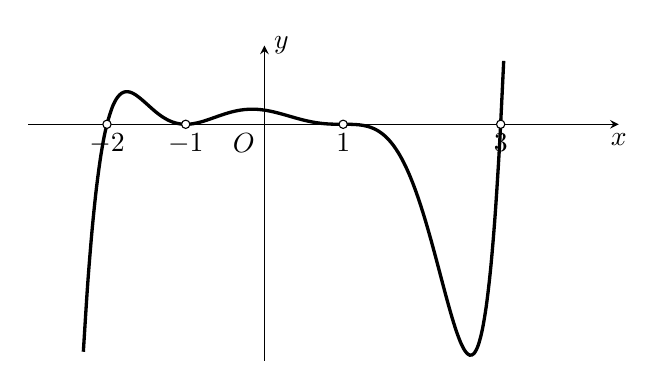
\begin{tikzpicture}[>=stealth]
    \draw[->](-3,0)--(4.5,0)node[below]{$x$};    
\draw[->](0,-3)--(0,1)node[right]{$y$};

\draw[domain=-2.3:3.04, smooth, samples=100, very thick]plot(\x, {0.03*(\x+2)*(\x+1)*(\x+1)*(\x-1)*(\x-1)*(\x-1)*(\x-3)});

\foreach \x in {-2,-1,1,3}
{
    \draw[fill=white](\x,0)node[below]{$\x$}circle(1.5pt);
}
\node [below left]{$O$};

\end{tikzpicture}
    \caption{}
\end{figure}
\end{analyze}

\begin{blk}
    如何解下列不等式:
    \begin{enumerate}[(1)]
        \item $(x+3)(x-2)(x^2-2x-3)<0$;
\item $(x-1)(x^2-x+5)>0$.
    \end{enumerate}
\end{blk}


\begin{example}
    解不等式:$(x+3)(x-2)^2(x+1)^2(x-1)\ge 0$.
\end{example}

\begin{analyze}
    这里出现了“$\ge $”。处理这类问题的办法是:在画函数图象的草图时,只要把曲线与$x$轴的交点画成“实点”即可。
\end{analyze}

\begin{solution}
    作出函数
$y=(x+3)(x-2)^2(x+1)^2(x-1)$的草图(图4.10)。

\begin{figure}[htp]
    \centering
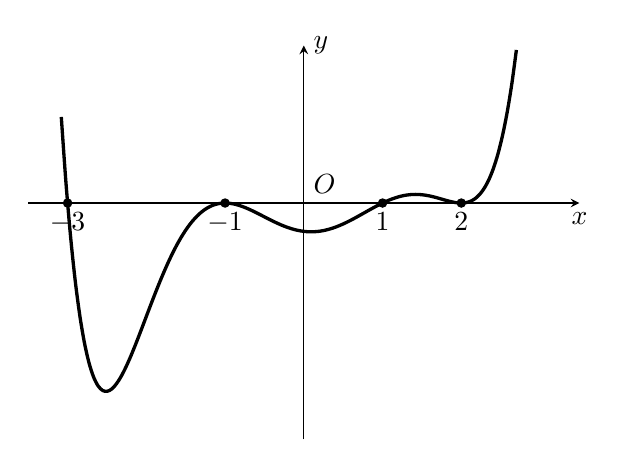
\begin{tikzpicture}[>=stealth]
    \draw[->](-3.5,0)--(3.5,0)node[below]{$x$};    
\draw[->](0,-3)--(0,2)node[right]{$y$};

\draw[domain=-3.08:2.7, smooth, samples=100, very thick]plot(\x, {0.03*(\x-2)*(\x-2)*(\x+1)*(\x+1)*(\x+3)*(\x-1)});

\foreach \x/\y in {-3,-1,1,2}
{
    \draw[fill](\x,0)node[below]{$\x$}circle(1.5pt);
}
\node [above right]{$O$};
\end{tikzpicture}
    \caption{}
\end{figure}

$\therefore\quad $不等式的解集是$(-\infty,-3]\cup\{-1\}\cup [1,+\infty)$
\end{solution}

\section*{习题十}
\begin{center}
    \bfseries A
\end{center}

\begin{enumerate}
    \item 解下列二次不等式:
\begin{multicols}{2}
\begin{enumerate}[(1)]
    \item $x^2+4x-45\ge 0$
    \item $x^2-5ax+6a^2>0$
\end{enumerate}
\end{multicols}

\item \begin{enumerate}[(1)]
    \item 解关于$x$的不等式:$ax^2-2ax+a+3\le 0$
\item 关于$x$的不等式$ax^2+5x+b>0$的解集是$\left(\frac13,\frac12\right)$
,求$a,b$

\item 关于$x$的不等式$ax^2+bx+c>0$ 的解集为$(\alpha,\beta)$, $\alpha >0$, 求关于$x$的不等式$cx^2+bx+a<0$的解集。
\end{enumerate} 

\item 解下列不等式组:
\begin{multicols}{2}
\begin{enumerate}[(1)]
    \item $\begin{cases}
        x^2-3x+2>0\\ x^2-2x-3\le 0
    \end{cases}$
    \item $\begin{cases}
        x-a\ge 0\\ x^2-2x-3<0
    \end{cases}$
\end{enumerate}
\end{multicols}
\item $a$为何值时,不等式组$\begin{cases}
    (x-2)(x-5)\le 0\\ x(x-a)\ge 0
\end{cases}$
的解集为:
\begin{multicols}{2}
\begin{enumerate}[(1)]
    \item $\emptyset$;
    \item 单元素集;
    \item 与第一个不等式同解.
\end{enumerate}
\end{multicols}

\item 解下列高次不等式:
\begin{enumerate}[(1)]
    \item $(x+2)(x^{2}-1)>0$;
    \item $(2x+1)(3x-1)(2-x)\leq 0$;
    \item $(x+1)^{3}(x-5)(x^{2}+3x)(x-2)^{2}(2x+1)^{2}<0$;
    \item $x^{2}(x+3)(x-1)(x-2)^{2}(x-3)\ge 0$.
\end{enumerate}

\item 不等式$ax^2+ax+(a-1)<0$对所有的实数$x$都成立,求$a$的取值范围.
\end{enumerate}

\begin{center}
    \bfseries B
\end{center}

\begin{enumerate}\setcounter{enumi}{6}
    \item 已知$M= \{ x\mid x^{2}- 3x- 10\ge 0\} $,
    $N=\{x\mid x^{2}-(2a+3)x+a^{2}+3a<0\}$.

    求$a$的值,使得:(1)$M\cap N=\emptyset$,\qquad (2)$M\cap N=N$.
    
    \item  不等式组$\begin{cases}x^{2}-x-2>0,\\2x^{2}+(2k+5)x+5k<0,\end{cases}$
    的整数解只有$-2$,求$k$的取值范围。
    
    \item  已知不等式$x^{2}-x-6<0$, $x^{2}+2x-8>0$, $x^{2}-4ax+3a^{2}<0$的解集分别是$A,B,C$.
    \begin{enumerate}[(1)]
        \item 试求$a$的取值范围,使$C\supseteq A\cap B$,
        \item 试求$a$的取值范围,使$C\supseteq \overline{A}\cap \overline{B}$.
    \end{enumerate}
    \item 设$A=\{x\mid (x+2)(x-1)>0\}$, $B=\{x\mid ax^2+abx+b\ge 0, \; a\ne 0\}$. 若$A\cap B=\emptyset$,且$A\cup B=A$,求$a$与$b$的关系.
\end{enumerate}

\begin{center}
    \bfseries C
\end{center}

\begin{enumerate}\setcounter{enumi}{10}
    \item 解关于$x$的不等式$ax^2-1<x+a$.
\end{enumerate}

\section{分式不等式的解法}

分母中含有未知数的不等式称为\textbf{分式不等式}。如
\[\frac{1}{x}<2,\qquad \frac{2x+3}{x-1}>x+1\]

解分式不等式的依据是4.10节中的定理4,其基本思想是将分式不等式“\textbf{化归}”与它同解的整式不等式,从而求出它的解集。

\begin{example}
    解不等式$\frac{2x-1}{(x+2)(x-3)}<0$.
\end{example}

\begin{solution}
  \[\text{原不等式}\Longleftrightarrow (2x-1)(x+2)(x-3)<0\]  

$\therefore\quad $解集为$(-\infty,-2)\cup\left(\frac{1}{2},3\right)$.(图4.11)
\end{solution}

\begin{example}
    解不等式$\frac{x^2+x-2}{x^3+7x^2-8x}\ge 0$.
\end{example}

\begin{solution}
    \[\text{原不等式}\Longleftrightarrow \frac{(x+2)(x-1)}{x(x+8)(x-1)}\ge 0 \Longleftrightarrow \begin{cases}
        (x+2)(x-1)^2 x(x+8)\ge 0\\
        x(x+8)(x-1)\ne 0
    \end{cases}   \]  

  $\therefore\quad $原不等式的解集是$(-8,-2]\cup(0,1)\cup (1,+\infty)$.(图4.12)
  \end{solution}

\begin{figure}[htp]
    \centering
\begin{minipage}{.4\textwidth}
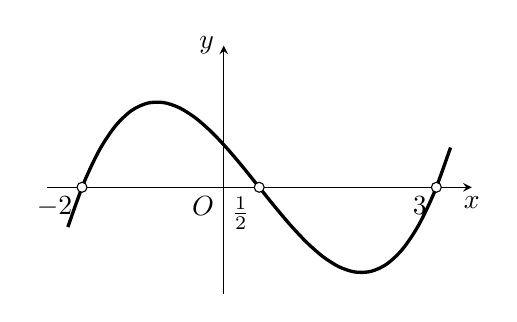
\begin{tikzpicture}[>=stealth,scale=.9]
\draw[->](-2.5,0)--(3.5,0)node[below]{$x$};
\draw[->](0,-1.5)--(0,2)node[left]{$y$};
\draw[domain=-2.2:3.2, smooth, very thick]plot(\x, {0.1*(\x+2)*(\x-3)*(2*\x-1)});
\foreach \x in {-2,3}
{
    \draw[fill=white](\x, 0)circle (2pt)node[below left]{$\x$};
}
\draw[fill=white](.5, 0)circle (2pt)node[below left]{$\frac{1}{2}$};
\node[below left]{$O$};
\end{tikzpicture}
\caption{}
\end{minipage}    \hfill
\begin{minipage}{.5\textwidth}
    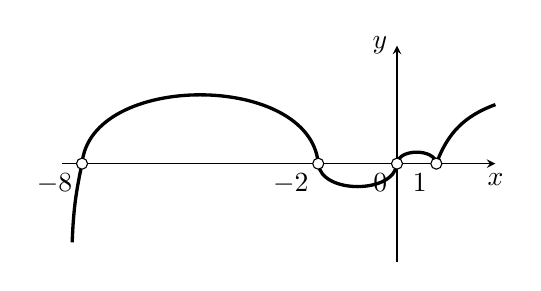
\begin{tikzpicture}[>=stealth, scale=.5]
\draw[->](-8.5,0)--(2.5,0)node[below]{$x$};
\draw[->](0,-2.5)--(0,3)node[left]{$y$};

\draw[very thick](-8.25,-2)[bend left=5] to (-8,0)[bend left=85]to (-2,0)[bend left=-85] to (0,0)[bend left=85] to (1,0)[bend left=25] to (2.5,1.5);
\foreach \x in {-2,0,1,-8}
{
    \draw[fill=white](\x, 0)circle (4pt)node[below left]{$\x$};
}
    \end{tikzpicture}
    \caption{}
    \end{minipage}    
\end{figure}

\begin{example}
解不等式$\frac{4}{x-1}\le x-1$.
\end{example}

\begin{solution}
\[\begin{split}
    \text{原不等式}&\Longleftrightarrow \frac{4}{x-1}-(x-1)\le 0 \Longleftrightarrow \frac{4-(x-1)^2}{x-1}\le 0\\
    &\Longleftrightarrow \frac{(3-x)(x+1)}{x-1}\le 0 \Longleftrightarrow \frac{(x-3)(x+1)}{x-1}\ge 0\\
    &\Longleftrightarrow \begin{cases}
        (x-3)(x+1)(x-1)\ge 0\\
        x-1\ne 0
    \end{cases}
\end{split}\]

$\therefore\quad $原不等式的解集是$[-1,0)\cup[3,+\infty)$. (图4.13)
\end{solution}

\begin{figure}[htp]
    \centering
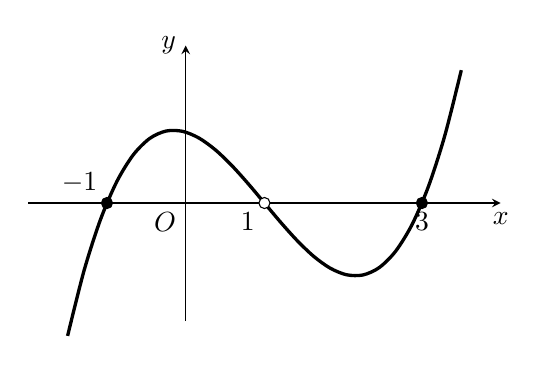
\begin{tikzpicture}[>=stealth]
    \draw[->](-2,0)--(4,0)node[below]{$x$};
    \draw[->](0,-1.5)--(0,2)node[left]{$y$};
    \draw[domain=-1.5:3.5, smooth, very thick]plot(\x, {0.3*(\x+1)*(\x-3)*(\x-1)});
    \foreach \x in {-1,3}
    {
        \draw[fill](\x, 0)circle (2pt);
    }
    \draw[fill=white](1, 0)circle (2pt)node[below left]{1};
    \node at (-1,0)[above left]{$-1$};
    \node at (3,0)[below]{$3$};
\node [below left]{$O$};
\end{tikzpicture}
    \caption{}
\end{figure}

\begin{example}
    解不等式$3x+5+\frac{1}{x-4}>2x+\frac{1}{x-4}+3$.
\end{example}

\begin{analyze}
    先消去不等号两边的分式将使解法简化,但消去后的不等式与原不等式不同解,这一点必须特别注意.
\end{analyze}

\begin{solution}
\[\text{原不等式}\Longleftrightarrow \begin{cases}
    3x+5>2x+3\\ x-4\ne 0
\end{cases} \Longleftrightarrow \begin{cases}
    x>-2\\ x\ne 4
\end{cases}\]

$\therefore\quad $原不等式的解集为$(-2,4)\cup (4,+\infty)$.
\end{solution}

\begin{example}
    解不等式$\frac{x-a}{(x+2)(x-3)}<0$\hfill (1)
\end{example}

\begin{solution}
\begin{equation}
    (1)\Longleftrightarrow (x-a)(x+2)(x-3)<0 \tag{2}
\end{equation}

由于$a$的不同取值使方程$(x-a)(x+2)(x-3)=0$的根在$x$轴上的相对位置不确定,故应对字母$a$的取值进行讨论。

\begin{figure}[htp]
    \centering
\begin{minipage}{.45\textwidth}
\begin{tikzpicture}[>=stealth, scale=.75]
\draw[->](-2.5,0)--(5.5,0)node[below]{$x$};
\draw[->](0,-1.5)--(0,3)node[left]{$y$};

\draw(-2.5,-1)[bend left=20] to (-2,0) [bend left=60] to (3,0)[bend right=30] to (4,0)[bend right=20] to (4.8,1.5);


\foreach \x in {-2,3}
{
    \draw[fill=white](\x, 0)circle (2pt)node[below]{$\x$};
}
\draw[fill=white](4, 0)circle (2pt)node[below]{$a$};
\node[below right]{$O$};
\end{tikzpicture}
\caption{}
\end{minipage}    \hfill
\begin{minipage}{.45\textwidth}
    \begin{tikzpicture}[>=stealth, scale=.75]
\draw[->](-2.5,0)--(5.5,0)node[below]{$x$};
\draw[->](0,-1.5)--(0,3)node[left]{$y$};

\draw(-2.5,-1)[bend left=20] to (-2,0) [bend left=60] to (3,0)[bend right=-30] to (4.8,1.5);


\foreach \x in {-2,3}
{
    \draw[fill=white](\x, 0)circle (2pt)node[below]{$\x$};
}
\node[below right]{$O$};
    \end{tikzpicture}
    \caption{}
    \end{minipage}    
\end{figure}


\begin{enumerate}[(i)]
    \item 当$a>3$时(图4.14),解集为$(-\infty,-2)\cup (3,a)$
    \item 当$a=3$时(图4.15),(2)变成$(x-3)^2(x+2)<0$
    
    $\therefore\quad $解集为$(-\infty,-2)$.
    \item 当$-2<a<3$时(图4.16),解集为$(-\infty,-2)\cup (a,3)$
    \item 当$a=-2$时(图4.17),(2)变成$(x+2)^2(x-3)<0$,解集为$(-\infty,-2)\cup (-2,3)$

\begin{figure}[htp]
    \centering
\begin{minipage}{.45\textwidth}
\begin{tikzpicture}[>=stealth, scale=.75]
\draw[->](-2.5,0)--(4.5,0)node[below]{$x$};
\draw[->](0,-1.5)--(0,3)node[left]{$y$};

\draw(-2.5,-1)[bend left=20] to (-2,0) [bend left=60] to (2,0)[bend right=30] to (3,0)[bend right=20] to (3.8,1);


\foreach \x in {-2,3}
{
    \draw[fill=white](\x, 0)circle (2pt)node[below]{$\x$};
}
\draw[fill=white](2, 0)circle (2pt)node[below]{$a$};
\node[below right]{$O$};
\end{tikzpicture}
\caption{}
\end{minipage}    \hfill
\begin{minipage}{.45\textwidth}
    \begin{tikzpicture}[>=stealth, scale=.75]
\draw[->](-3,0)--(5,0)node[below]{$x$};
\draw[->](0,-2.5)--(0,2)node[left]{$y$};

\draw(-2.75,-.75)[bend left=-20] to (-2,0) [bend right=60] to (3,0)[bend right=10] to (4.5,1.5);


\foreach \x in {-2,3}
{
    \draw[fill=white](\x, 0)circle (2pt);
}
\node[below left]{$O$};
\node at (-2,0)[above]{$-2$};
\node at (3,0)[below]{$3$};


    \end{tikzpicture}
    \caption{}
    \end{minipage}    
\end{figure}
    \item 当$a<-2$时(图4.18),解集为$(-\infty,a)\cup (-2,3)$
\end{enumerate}

\begin{figure}[htp]
    \centering
\begin{tikzpicture}[>=stealth, scale=.8]
\draw[->](-6,0)--(4.5,0)node[below]{$x$};
\draw[->](0,-2)--(0,1.5)node[left]{$y$};

\draw(-5.5,-1)[bend left=20] to (-5,0) [bend left=50] to (-2,0)[bend right=50] to  (3,0)[bend left=-20] to (3.5,1);

\draw[fill=white](-2, 0)circle (2pt)node[below left]{$-2$};
\draw[fill=white](-5, 0)circle (2pt)node[below]{$a$};
\draw[fill=white](3, 0)circle (2pt)node[below]{$3$};
\node[above right]{$O$};
\end{tikzpicture}
    \caption{}
\end{figure}

\end{solution}

\section*{习题十一}
\begin{center}
    \bfseries A
\end{center}

\begin{enumerate}
    \item 解下列不等式:
\begin{multicols}{2}
\begin{enumerate}[(1)]
    \item $3x-2+\frac{1}{5-x}>2x+1-\frac{1}{x-5}$
    \item $\frac{2x-3}{3x-4}<2$
    \item $\frac{x(x-3)}{x^2-3x+2}<0$
    \item $\frac{x^2}{x^2-6x+8}\ge 1$
    \item $\frac{x+1}{(x-2)^2 (x+1)}<1$
    \item $2+\frac{2}{x-1}\le \frac{5}{4-x}$
\end{enumerate}
\end{multicols}

\item (选择题)下列不等式中,与$\frac{x-3}{2-x}\ge 0$同解的是(\qquad )
\begin{multicols}{2}
\begin{enumerate}[(A)]
    \item $(x-3)(2-x)\ge 0$
    \item $(x-3)(2-x)>0$
    \item $\frac{2-x}{x-3}\ge 0$
    \item $\lg(x-2)\le 0$
\end{enumerate}
\end{multicols}
\end{enumerate}

\begin{center}
    \bfseries C
\end{center}
\begin{enumerate}
 \setcounter{enumi}{2}   
 \item 解关于$x$的不等式$5^{\tfrac{a(1-x)}{x-2}+1}<1$
\end{enumerate}

\section{无理不等式的解法}
在根号内含有未知数的不等式称为\textbf{无理不等式}。如$\sqrt{x-1}>x-3$, $\sqrt{x}+2<\sqrt{2x-1}+1$等.

解无理不等式应注意:
\begin{enumerate}[(1)]
\item 必须使出现在不等式中的根式有意义,这就需要求出根式中函数的定义域;
\item 无理不等式的求解,根本是\textbf{化归}为有理不等式,转化的依据是4.10节中的定理5。
\end{enumerate}

以下研究几个例子。

\begin{example}
解不等式$\sqrt{x-1}>x-3$\hfill (1)
\end{example}

\begin{analyze}
\begin{enumerate}
    \item 为使用定理5,应对有理式$x-3$进行讨论。
    \item (1)式的结构特征使我们想到换元法。
    \item (1)式两边都是我们熟知的函数。
\end{enumerate}
\end{analyze}


\begin{solution}
\textbf{解法1:}
\[(1)\Longleftrightarrow {\rm (I)}\begin{cases}
    x-3\ge 0& \text{(限制条件)}\\
x-1\ge 0 &\text{(定义域)}\\
x-1>(x-3)^2
\end{cases} \text{和}\quad {\rm (II)}\begin{cases}
    x-3<0& \text{(限制条件)}\\
    x-1\ge 0 &\text{(定义域)}\\
\end{cases}\]
而
\[{\rm (I)}\Longleftrightarrow \begin{cases}
    x\ge 3\\
    x-1>(x-3)^2
\end{cases}\Longleftrightarrow \begin{cases}
    x\ge 3\\
    (x-2)(x-5)<0
\end{cases}\]
$\therefore\quad 3\le x<5$.

\[{\rm (II)}\Longleftrightarrow \begin{cases}
    x< 3\\
    x\ge 1
\end{cases}\qquad \therefore\quad 1\le x<3\]

$\therefore\quad $(1)的解集为$[3,5)\cup[1,3)$,即$[1,5)$.

\textbf{解法2:}
(1)即$\sqrt{x-1}>(x-1)-2$.

令$t=\sqrt{x-1}\ge 0$,得$\begin{cases}
    t\ge 0\\t^2-t-2<0
\end{cases}$

解之,得$0\le t<2$,即$0\le \sqrt{x-1}<2\Longleftrightarrow \begin{cases}
    x-1\ge 0\\ x-1<4
\end{cases}$

$\therefore\quad 1\le x<5$.

\textbf{解法3:}
令$y_1=\sqrt{x-1}$,$y_2=x-3$,从而(1)的解集就是使函数$y_1>y_2$的$x$的取值范围。在同一个坐标系中分别作出两个函数的图象(图4.19). 设它们交点的横坐标是$x_0$,则$\sqrt{x_0-1}=x_0-3>0$

解之,得$x_0=2$(舍)或$x_0=5$

$\therefore\quad $(1)的解集为$[1,5)$.

\begin{figure}[htp]
    \centering
\begin{tikzpicture}[>=stealth, scale=.8]
\draw[->](-1,0)--(7,0)node[below]{$x$} ;   
\draw[->](0,-4)--(0,4)node[left]{$y$} ;
\draw[domain=1:6, smooth, samples=100, very thick]plot(\x, {sqrt(\x-1)})node[right]{$y_1=\sqrt{x-1}$};
\draw[domain=-.5:6, smooth, very thick]plot(\x, {\x-3});
\node at (1.5,-2)[right]{$y_2=x-3$};
\foreach \x in {-3,-2,-1,1,2,3}
{
    \draw(0,\x)--(.1,\x);
}
\foreach \x in {1,3}
{
    \draw(\x,0)node[below]{\x}--(\x,.1);
}
\draw[dashed](5,0)node[below]{$x_0$}--(5,2);
\node [below left]{$O$};

\draw[fill](1,0) circle (2pt);

\end{tikzpicture}
    \caption{}
\end{figure}

\end{solution}

\begin{rmk}
解法1是通法,应熟练掌握。换元法与图象法的突破口是认清式子的结构特征。
\end{rmk}

\begin{example}
解不等式$(x-1)\sqrt{x+2}\ge 0$\hfill (1)
\end{example}

\begin{solution}
\[(1)\Longleftrightarrow \begin{cases}
    (x-1)\sqrt{x+2}>0& (2)\\
    (x-1)\sqrt{x+2}=0 & (3)
\end{cases}\]
\[(2)\Longleftrightarrow \begin{cases}
    x+2\ge 0\\ x-1>0 
\end{cases}\qquad \therefore\quad x>1\]
(3)的解集是$x=1$或$x=-2$.

$\therefore\quad $(1)的解集为$[1,+\infty)\cup\{-2\}$.
\end{solution}

\begin{example}
解不等式$\sqrt{2ax-a^2}>a-x\; (a>0)$\hfill (1)
\end{example}

\begin{solution}
\[(1)\Longleftrightarrow {\rm (I)}\begin{cases}
    a-x\ge 0\\
    2ax-a^2\ge 0\\
    2ax-a^2>(a-x)^2
\end{cases}\text{和}\quad {\rm (II)}\begin{cases}
    a-x<0\\ 2ax-a^2\ge 0
\end{cases}\]
而
\[\begin{split}
{\rm (I)}&\Longleftrightarrow \begin{cases}
    a-x\ge 0\\ 2ax-a^2>(a-x)^2
\end{cases}\Longleftrightarrow \begin{cases}
    x\le a\\(x-2a)^2<2a^2
\end{cases}\\
&\Longleftrightarrow \begin{cases}
    x\le a\\|x-2a|<\sqrt{2}a
\end{cases}\Longleftrightarrow \begin{cases}
    x\le a\\ 2a-\sqrt{2}a<x\le 2a+\sqrt{2}a
\end{cases}
\end{split}\]
$\therefore\quad 2a-\sqrt{2}a<x\le a\quad (\because\quad a>0)$

\[{\rm (II)}\Longleftrightarrow \begin{cases}
    x>a\\ x\ge \frac{a}{2}
\end{cases}\qquad \therefore\quad x>a\quad (\because \quad a>0)\]
$\therefore\quad $(1)的解集是$(2a-\sqrt{2}a,a]\cup (a,+\infty)=\left((2-\sqrt{2})a,+\infty\right)$
\end{solution}


\section*{习题十二}
\begin{center}
    \bfseries A
\end{center}
解下列不等式(1—8题)
\begin{enumerate}
    \item $4x-3+\sqrt{10-x}>3x+2+\sqrt{10-x}$
    \item $\sqrt{3-x}>x-2$
    \item $\sqrt{2x^{2}-6x+4}<x+2$
    \item $\sqrt{3x-15}-\sqrt{x-4}\ge 0$
    \item $\sqrt{4-\log_{0.3}x}<\log_{0.3}x-2$ (提示:令$\log_{0.3}x=y$)
    \item $\sqrt{x-2}-\sqrt{x-5}>1$
\end{enumerate}


\begin{center}
    \bfseries B
\end{center}

\begin{enumerate}\setcounter{enumi}{6}
    \item $\sqrt{\log_{2}^{2}x+\log_{2}x-2}> 2\log_{2}x-2$
    \item $(x-1)\sqrt{x^{2}-x-2}\ge 0$
    \item 设$A= \{ x\mid 5- x> \sqrt {2(x- 1) }\}$, 
$B=\left\{x\mid x^{2}-ax\le x-a\right\}$,
要使$A\subset B$, 求实数$a$的取值范围。
\item 解关于$x$的不等式$\sqrt{2x-a}<\sqrt{x+1}$
\end{enumerate}


\begin{center}
    \bfseries C
\end{center}

\begin{enumerate}\setcounter{enumi}{10}
    \item 解关于$x$的不等式$\sqrt{a-2x}>a-x$(提示:参考例1的解法2).
\end{enumerate}

\section{绝对值不等式的性质、解法与证明}

在绝对值符号中含有未知数的不等式称为\textbf{绝对值不等式}。如
$|x-2|<3$, $|x-1|-|x+2|\ge 5$等。

\begin{thm}{实数绝对值的定义}
若$a\in\R$,那么
\[|a|=\begin{cases}
    a, &a>0\\
    0, &a=0\\
    -a, &a<0\\
\end{cases}\]
显然有$$-|a|\le a\le |a|$$
\end{thm}

\begin{thm}
    {最简绝对值不等式的解集(填空)}
\begin{enumerate}[(1)]
\item 若$|x|<R$,则$x\in \blank$;
\item 若$|x|>r,\; (r>0)$,则$x\in\blank$;
\item 若$r<|x|<R,\; (0<r<R)$,则$x\in\blank$.
\end{enumerate}
\end{thm}

\begin{note}
\begin{enumerate}[(i)]
    \item 若把$x$看作数轴上点$P$的坐标,则$|x|$就是点$P$到原点$O$的距离。那么,上述三个最简绝对值不等式的解集的几何意义十分明显。
    \item 把三个最简绝对值不等式写成与它等价的解集的形式是脱去绝对值符号的重要方法,应该熟练掌握。
    \item 为了“脱去”绝对值号,有时也采用不等式两边分别平方的办法。如
\[|A|\ge |B|\Longleftrightarrow A^2\ge B^2\]
(这是因为$|A|\ge |B|\ge 0$)
\item 这里的正数$R$、$r$不仅可以放宽到零和负数,而且进一步还可以放宽为含未知数的解析式(这无疑会给解题带来极大的方便):
\begin{itemize}
    \item 推广1:$|x|<\varphi(x)\Longleftrightarrow -\varphi(x)<x<\varphi(x)$;
    \item 推广2:$|x|>\varphi(x)\Longleftrightarrow x<-\varphi(x)\text{或}x>\varphi(x)$.
\end{itemize}
(用5.11中定理1的证法可以证明这两个推广)
\end{enumerate}
\end{note}

\begin{example}
解不等式$|x^2+3x-8|\le 10$\hfill (1)
\end{example}

\begin{solution}
    $(1)\Longleftrightarrow -10\le x^2+3x-8\le 10 $\hfill (2)
\[\begin{split}
  (2) & \Longleftrightarrow \begin{cases}
        -10\le x^2+3x-8\\
        x^2+3x-8\le 10
    \end{cases}
     \Longleftrightarrow \begin{cases}
        x^2+3x+2\ge 0\\
        x^2+3x-18\le 0
    \end{cases}\\
    &\Longleftrightarrow \begin{cases}
        (x+2)(x+1)\ge 0,&(3)\\
        (x+6)(x-3)\le 0,&(4)
    \end{cases}
\end{split}\]

很清楚(图4.20), 不等式组(3)、(4)的解集为$[-6,-2]\cup [-1,3]$.
\end{solution}

\begin{figure}[htp]
    \centering
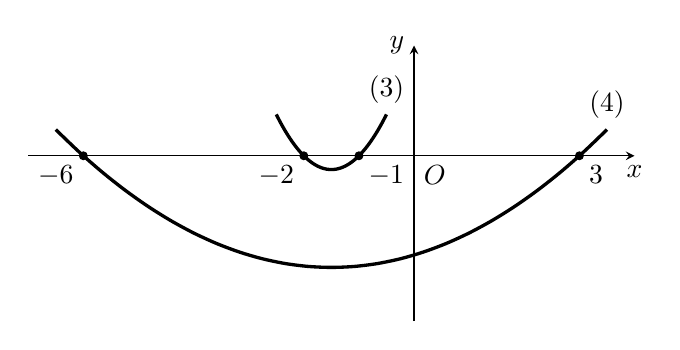
\begin{tikzpicture}[>=stealth, scale=.7]
\draw[->](-7,0)--(4,0)node[below]{$x$} ;   
\draw[->](0,-3)--(0,2)node[left]{$y$} ;
\draw[domain=-2.5:-.5, smooth, very thick]plot(\x, {(\x+2)*(\x+1)})node[above]{$(3)$};
\draw[domain=-6.5:3.5, smooth, very thick]plot(\x, {0.1*(\x+6)*(\x-3)})node[above]{$(4)$};
\foreach \x in {-6,-2}
{
    \node at (\x,0)[below left]{$\x$};
    \draw[fill](\x,0) circle(2pt);
}
\foreach \x in {-1,3}
{
    \node at (\x,0)[below right]{$\x$};
    \draw[fill](\x,0) circle(2pt);
}
\node[below right]{$O$};
\end{tikzpicture}
    \caption{}
\end{figure}

\begin{example}
    解不等式$|5x-x^2|>6$\hfill (1)
\end{example}

\begin{solution}
(1)即 $|x^2-5x|>6$\hfill (*)

(习惯上,我们总是先按x的降幂排列,并使x的最高次项的系数为正)。

\[\begin{split}
    (*)&\Longleftrightarrow x^2-5x<-6,\text{或}x^2-5x>6 \\
    &\Longleftrightarrow x^2-5x+6<0,\text{或}x^2-5x-6>0\Longleftrightarrow \begin{cases}
        (x-2)(x-3)<0,& (2)\\
        (x-6)(x+1)>0,& (3)
    \end{cases}
\end{split} \]
(2)的解集是$(2,3)$;(3)的解集是$(-\infty,-1)\cup (6,+\infty)$.

$\therefore\quad (1)$的解集为$(2,3)\cup (-\infty,-1)\cup (6,+\infty)$
\end{solution}

\begin{example}
    解不等式$3\le |5-2x|<9$\hfill (1)
\end{example}

\begin{solution}
先把(1)改写成 $3\le |2x-5|<9$\hfill (*)

根据最简绝对值不等式(3),有
\[(*)\Longleftrightarrow \begin{cases}
    -9< 2x-5\le -3,& (2)\\
    3\le 2x-5<9,&(3)
\end{cases}\]

$\therefore\quad (1)$的解集为$(-2,1]\cup[4,7)$.
\end{solution}

\begin{rmk}
上述三例,都是利用最简绝对值不等式的解集脱去了绝对值符号,这是最常用也是最基本的方法。若要用“先平方”的办法脱去绝对值号,运算量一般都较大,而且有时还有可能增解,这时必须检验。
\end{rmk}

\begin{example}
    解不等式$\left|x^2-4\right|\le  x+2$\hfill (1)
\end{example}

\begin{solution}
    根据推广1,$(1)\Longleftrightarrow-x-2\le  x^{2}-4\le  x+2$
即
\[\begin{cases}x^{2}-4\geqslant-x-2,\\
    x^{2}-4\leqslant x+2,
\end{cases}\Longleftrightarrow
\begin{cases}
    x^{2}+x-2\geqslant0,\\
    x^{2}-x-6\leqslant0,
\end{cases}\Longleftrightarrow\begin{cases}(x+2)(x-1)\geqslant0,\\
    (x+2)(x-3)\leqslant0.
\end{cases}\]
$\therefore\quad $ (1)的解集为$[1,3]\cup \{-2\}$.
\end{solution}

\begin{thm}{思考题}
    用图象法解此题行吗?试一试。
\end{thm}

\begin{example}
    解不等式$\left|\frac{x+3}{2x-1}\right|\leqslant1$
\end{example}

\begin{solution}
\textbf{解法1:}原不等式同解于:
\[\begin{split}
    &|x+3|\leqslant|2x-1|, \text{ 且 } 2x-1\neq0,\\
&\Longleftrightarrow (x+3)^{2}\leqslant(2x-1)^{2}\text{ 且 }2x-1\neq0,\\
&\Longleftrightarrow 3x^{2}-10x-8\geqslant 0\text{ 且 }2x-1\neq0\\
&\Longleftrightarrow(3x+2)(x-4)\geqslant0\text{ 且 }2x-1\neq0.
\end{split}\]

$\therefore\quad $(1)的解集为$\left(-\infty,-\frac23\right]\cup[4,+\infty)$.    

\textbf{解法2:}
\[\begin{split}
    (1)&\Longleftrightarrow \left(\frac{x+3}{2x-1}\right)^2-1\le 0\\
    &\Longleftrightarrow \frac{3x^2-10x-8}{(2x-1)^2}\ge 0 \Longleftrightarrow \begin{cases}
        (3x+2)(x-4)\ge 0\\
        (2x-1)^2\ne 0
    \end{cases}
\end{split} \]
$\therefore\quad $(1)的解集为$\left(-\infty,-\frac{2}{3}\right]\cup [4,+\infty)$.
\end{solution}

\begin{example}
    解不等式$|x+7|-|x-2|<3$\hfill (1)
\end{example}

\begin{analyze}
这里出现了两个绝对值号,上述三个最简绝对值不等式的结果已不能使用,只好根据“实数绝对值的定义”去脱绝对值号。为此,需要分别求出$|x+7|$与$|x-2|$的零点(使函数值为零的$x$值),再以诸零点为边界,把$(-\infty,+\infty)$分成几个相互连接的区间,然后在每个区间上去探求(1)的解。也就是说,把在实数集$\R$上解不等式(1),转化成在
$\R$的子区间上分别去解(1)。这就是此法的实质。

\end{analyze}

\begin{solution}
    由于$-7$, 2分别是$|x+7|$与$|x-2|$的零点,它们把区间$(-\infty,+\infty)$分成三个子区间(图4.21)。

\begin{figure}[htp]
    \centering
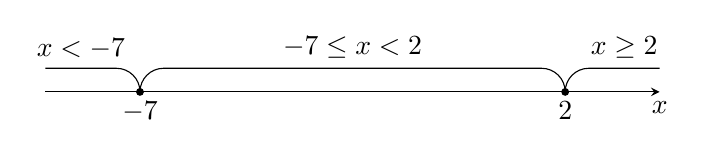
\begin{tikzpicture}[>=stealth, scale=.6]
    \draw[->](-9,0)--(4,0)node[below]{$x$};
\foreach \x in {-7,2}
{
    \node at (\x,0)[below]{$\x$};
    \draw[fill](\x,0) circle(2pt);
}    
\draw(-9,.5)--node[above]{$x<-7$}(-7.5,.5)[bend left=45] to (-7,0);
\draw(2,0)[bend left=-45] to (2-.5,.5)--node[above]{$-7\le x<2$}(-6.5,.5)[bend left=-45] to (-7,0);
\draw(4,.5)--node[above]{$x\ge 2$}(2.5,.5) [bend left=-45] to (2,0);
\end{tikzpicture}
    \caption{}
\end{figure}

由此,(1)可化成三个不等式组:
\begin{enumerate}[(1)]
    \item $\begin{cases}x\geqslant2,\\(x+7)-(x-2)<3,\end{cases}\Longleftrightarrow\begin{cases}x\geqslant2,\\9<3.\end{cases}$
    
    $\therefore\quad$ 解集$X_1=\emptyset$

    \item $\begin{cases} - 7\leq x< 2, \\ ( x+ 7) + ( x- 2) < 3, \end{cases} \Longleftrightarrow \begin{cases} - 7\leq x< 2, \\ x< - 1.  \end{cases}$
    
    $\therefore\quad$ 解集$X_2=[-7,-1)$
    
\item $\begin{cases} x< - 7, \\ - ( x+ 7) - [ - ( x- 2) ] < 3. 
\end{cases} 
\Longleftrightarrow \begin{cases} x< - 7, \\ - 9< 3. \end{cases}$

$\therefore\quad$ 解集$X_3=(-\infty,-7)$.
\end{enumerate}

$\therefore\quad$(1)的解集为$X_1\cup X_2\cup X_3=(-\infty,-1)$.
\end{solution}

\begin{thm}{思考题}
\begin{enumerate}[(1)]
    \item 根据(1)式的几何意义,你能通过画出数轴直接看出它的解集吗?
    \item 根据几何意义,你能判断不等式$|x|+|x-3|<1$无解吗?
\end{enumerate}
\end{thm}

\begin{example}
    解不等式$\frac{\log_{0.1}|x-2|}{x^2-4x}<0$\hfill (1)
\end{example}

\begin{solution}
\[\begin{split}
    (1)&\Longleftrightarrow \begin{cases}
        \log_{0.1}|x-2|>0\\
        x^2-4x<0
    \end{cases}\text{或}\quad \begin{cases}
        \log_{0.1}|x-2|<0\\
        x^2-4x>0
    \end{cases}\\
    &\Longleftrightarrow \begin{cases}
        0<|x-2|<1\\
        x(x-4)<0
    \end{cases}\text{(图4.22)\quad 或}\quad \begin{cases}
        |x-2|>1 \\
        x(x-4)>0
    \end{cases}\text{(图4.23)}\\
\end{split}\]

\begin{figure}[htp]
    \centering
\begin{minipage}{.45\textwidth}
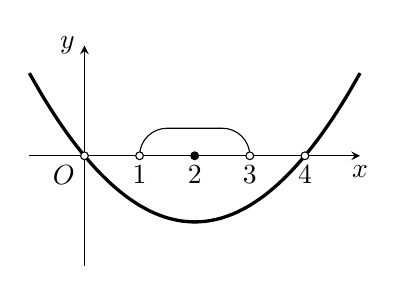
\begin{tikzpicture}[>=stealth, scale=.7]
\draw[->](-1,0)--(5,0)node[below]{$x$};
\draw[->](0,-2)--(0,2)node[left]{$y$};
\node[below left]{$O$};
\foreach \x in {1,2,3,4}
{
    \node at (\x,0)[below]{$\x$};
}
\draw(1,0)[bend left=45] to (1.5,.5)--(3-.5,.5)[bend left=45] to (3,0);
\draw[domain=-1:5, smooth, very thick]plot(\x, {0.3*\x*(\x-4)});

\foreach \x in {0,1,3,4}
{
    \draw[fill=white](\x,0)circle (2pt);
}
\draw[fill](2,0)circle (2pt);


\end{tikzpicture}
\caption{}
\end{minipage}
\hfill
\begin{minipage}{.45\textwidth}
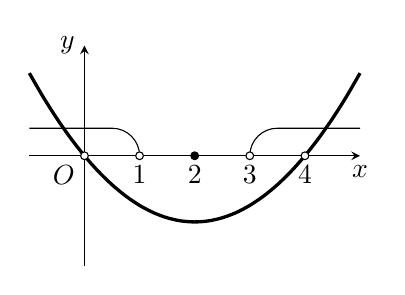
\begin{tikzpicture}[>=stealth, scale=.7]
    \draw[->](-1,0)--(5,0)node[below]{$x$};
    \draw[->](0,-2)--(0,2)node[left]{$y$};
    \node[below left]{$O$};
    \foreach \x in {1,2,3,4}
{
    \node at (\x,0)[below]{$\x$};
}
\draw(3,0)[bend left=45] to (3.5,.5)--(5,.5);
\draw(-1,.5)--(.5,.5)[bend left=45] to (1,0);
\draw[domain=-1:5, smooth, very thick]plot(\x, {0.3*\x*(\x-4)});

\foreach \x in {0,1,3,4}
{
    \draw[fill=white](\x,0)circle (2pt);
}
\draw[fill](2,0)circle (2pt);
\end{tikzpicture}
\caption{}
\end{minipage}
\end{figure}

$\therefore\quad $(1)的解集为$(1,2)\cup (2,3)\cup (-\infty,0)\cup (4,+\infty)$.

\end{solution}

\begin{example}
    用简捷方法解$|x^2-2|<|x|$ \hfill (1)
\end{example}

\begin{solution}
\textbf{解法1:}(1)即$\Big||x|^2-2\Big|<|x|$

令$|x|=y$,则上式$\Longleftrightarrow |y^2-2|<y\Longleftrightarrow 1<y<2$

$\therefore\quad 1<|x|<2$.

从而(1)的解集为$(-2,-1)\cup (1,2)$.

\textbf{解法2:} $\because\quad $不等号两边的函数都为偶函数,

$\therefore\quad $若$x$为(1)的解,则$-x$也为(1)的解。

当$x\ge 0$时,$(1)\Longleftrightarrow |x^2-2|<x$,
解之得$1<x<2$

$\therefore\quad $当$a\le 0$时,必有$-2<x<-1$, 
从而,(1)的解集为$(-2,-1)\cup (1,2)$.
\end{solution}

\section*{习题十三}
\begin{center}
    \bfseries A
\end{center}

\begin{enumerate}
    \item 解不等式:
\begin{multicols}{2}
\begin{enumerate}[(1)]
    \item $|x+1|<\sqrt{2}$
    \item $1<|x-4|\leqslant2$
    \item $| x^{2}-2x-3|-2>0$
    \item $3\leqslant|5-2x|<9$
    \item $|x^{2}+2x-1|<2$
    \item $|x^{2}-1|\geqslant x$
    \item $|x^{3}-1|>1-x$
\end{enumerate}
\end{multicols}

\item 解不等式:
\begin{multicols}{2}
\begin{enumerate}[(1)]
    \item $|x+6|-|3-2x|>4$
    \item $\sqrt{4-4x+x^{2}}+|x-3|-1\leq0$
    \item $\sqrt{x^{2}+2x+1}-2|2-x|>5-x$
    \item $|x|+|x-3|\leqslant1$
\end{enumerate}
\end{multicols}

\item 求$|x-a|+|x-b|+|x-c|$的最小值。(提示:从几何意义上考虑最简便)
\end{enumerate}





































































































































































